\documentclass[1p]{elsarticle_modified}
%\bibliographystyle{elsarticle-num}

%\usepackage[colorlinks]{hyperref}
%\usepackage{abbrmath_seonhwa} %\Abb, \Ascr, \Acal ,\Abf, \Afrak
\usepackage{amsfonts}
\usepackage{amssymb}
\usepackage{amsmath}
\usepackage{amsthm}
\usepackage{scalefnt}
\usepackage{amsbsy}
\usepackage{kotex}
\usepackage{caption}
\usepackage{subfig}
\usepackage{color}
\usepackage{graphicx}
\usepackage{xcolor} %% white, black, red, green, blue, cyan, magenta, yellow
\usepackage{float}
\usepackage{setspace}
\usepackage{hyperref}

\usepackage{tikz}
\usetikzlibrary{arrows}

\usepackage{multirow}
\usepackage{array} % fixed length table
\usepackage{hhline}

%%%%%%%%%%%%%%%%%%%%%
\makeatletter
\renewcommand*\env@matrix[1][\arraystretch]{%
	\edef\arraystretch{#1}%
	\hskip -\arraycolsep
	\let\@ifnextchar\new@ifnextchar
	\array{*\c@MaxMatrixCols c}}
\makeatother %https://tex.stackexchange.com/questions/14071/how-can-i-increase-the-line-spacing-in-a-matrix
%%%%%%%%%%%%%%%

\usepackage[normalem]{ulem}

\newcommand{\msout}[1]{\ifmmode\text{\sout{\ensuremath{#1}}}\else\sout{#1}\fi}
%SOURCE: \msout is \stkout macro in https://tex.stackexchange.com/questions/20609/strikeout-in-math-mode

\newcommand{\cancel}[1]{
	\ifmmode
	{\color{red}\msout{#1}}
	\else
	{\color{red}\sout{#1}}
	\fi
}

\newcommand{\add}[1]{
	{\color{blue}\uwave{#1}}
}

\newcommand{\replace}[2]{
	\ifmmode
	{\color{red}\msout{#1}}{\color{blue}\uwave{#2}}
	\else
	{\color{red}\sout{#1}}{\color{blue}\uwave{#2}}
	\fi
}

\newcommand{\Sol}{\mathcal{S}} %segment
\newcommand{\D}{D} %diagram
\newcommand{\A}{\mathcal{A}} %arc


%%%%%%%%%%%%%%%%%%%%%%%%%%%%%5 test

\def\sl{\operatorname{\textup{SL}}(2,\Cbb)}
\def\psl{\operatorname{\textup{PSL}}(2,\Cbb)}
\def\quan{\mkern 1mu \triangleright \mkern 1mu}

\theoremstyle{definition}
\newtheorem{thm}{Theorem}[section]
\newtheorem{prop}[thm]{Proposition}
\newtheorem{lem}[thm]{Lemma}
\newtheorem{ques}[thm]{Question}
\newtheorem{cor}[thm]{Corollary}
\newtheorem{defn}[thm]{Definition}
\newtheorem{exam}[thm]{Example}
\newtheorem{rmk}[thm]{Remark}
\newtheorem{alg}[thm]{Algorithm}

\newcommand{\I}{\sqrt{-1}}
\begin{document}

%\begin{frontmatter}
%
%\title{Boundary parabolic representations of knots up to 8 crossings}
%
%%% Group authors per affiliation:
%\author{Yunhi Cho} 
%\address{Department of Mathematics, University of Seoul, Seoul, Korea}
%\ead{yhcho@uos.ac.kr}
%
%
%\author{Seonhwa Kim} %\fnref{s_kim}}
%\address{Center for Geometry and Physics, Institute for Basic Science, Pohang, 37673, Korea}
%\ead{ryeona17@ibs.re.kr}
%
%\author{Hyuk Kim}
%\address{Department of Mathematical Sciences, Seoul National University, Seoul 08826, Korea}
%\ead{hyukkim@snu.ac.kr}
%
%\author{Seokbeom Yoon}
%\address{Department of Mathematical Sciences, Seoul National University, Seoul, 08826,  Korea}
%\ead{sbyoon15@snu.ac.kr}
%
%\begin{abstract}
%We find all boundary parabolic representation of knots up to 8 crossings.
%
%\end{abstract}
%\begin{keyword}
%    \MSC[2010] 57M25 
%\end{keyword}
%
%\end{frontmatter}

%\linenumbers
%\tableofcontents
%
\newcommand\colored[1]{\textcolor{white}{\rule[-0.35ex]{0.8em}{1.4ex}}\kern-0.8em\color{red} #1}%
%\newcommand\colored[1]{\textcolor{white}{ #1}\kern-2.17ex	\textcolor{white}{ #1}\kern-1.81ex	\textcolor{white}{ #1}\kern-2.15ex\color{red}#1	}

{\Large $\underline{12a_{0784}~(K12a_{0784})}$}

\setlength{\tabcolsep}{10pt}
\renewcommand{\arraystretch}{1.6}
\vspace{1cm}\begin{tabular}{m{100pt}>{\centering\arraybackslash}m{274pt}}
\multirow{5}{120pt}{
	\centering
	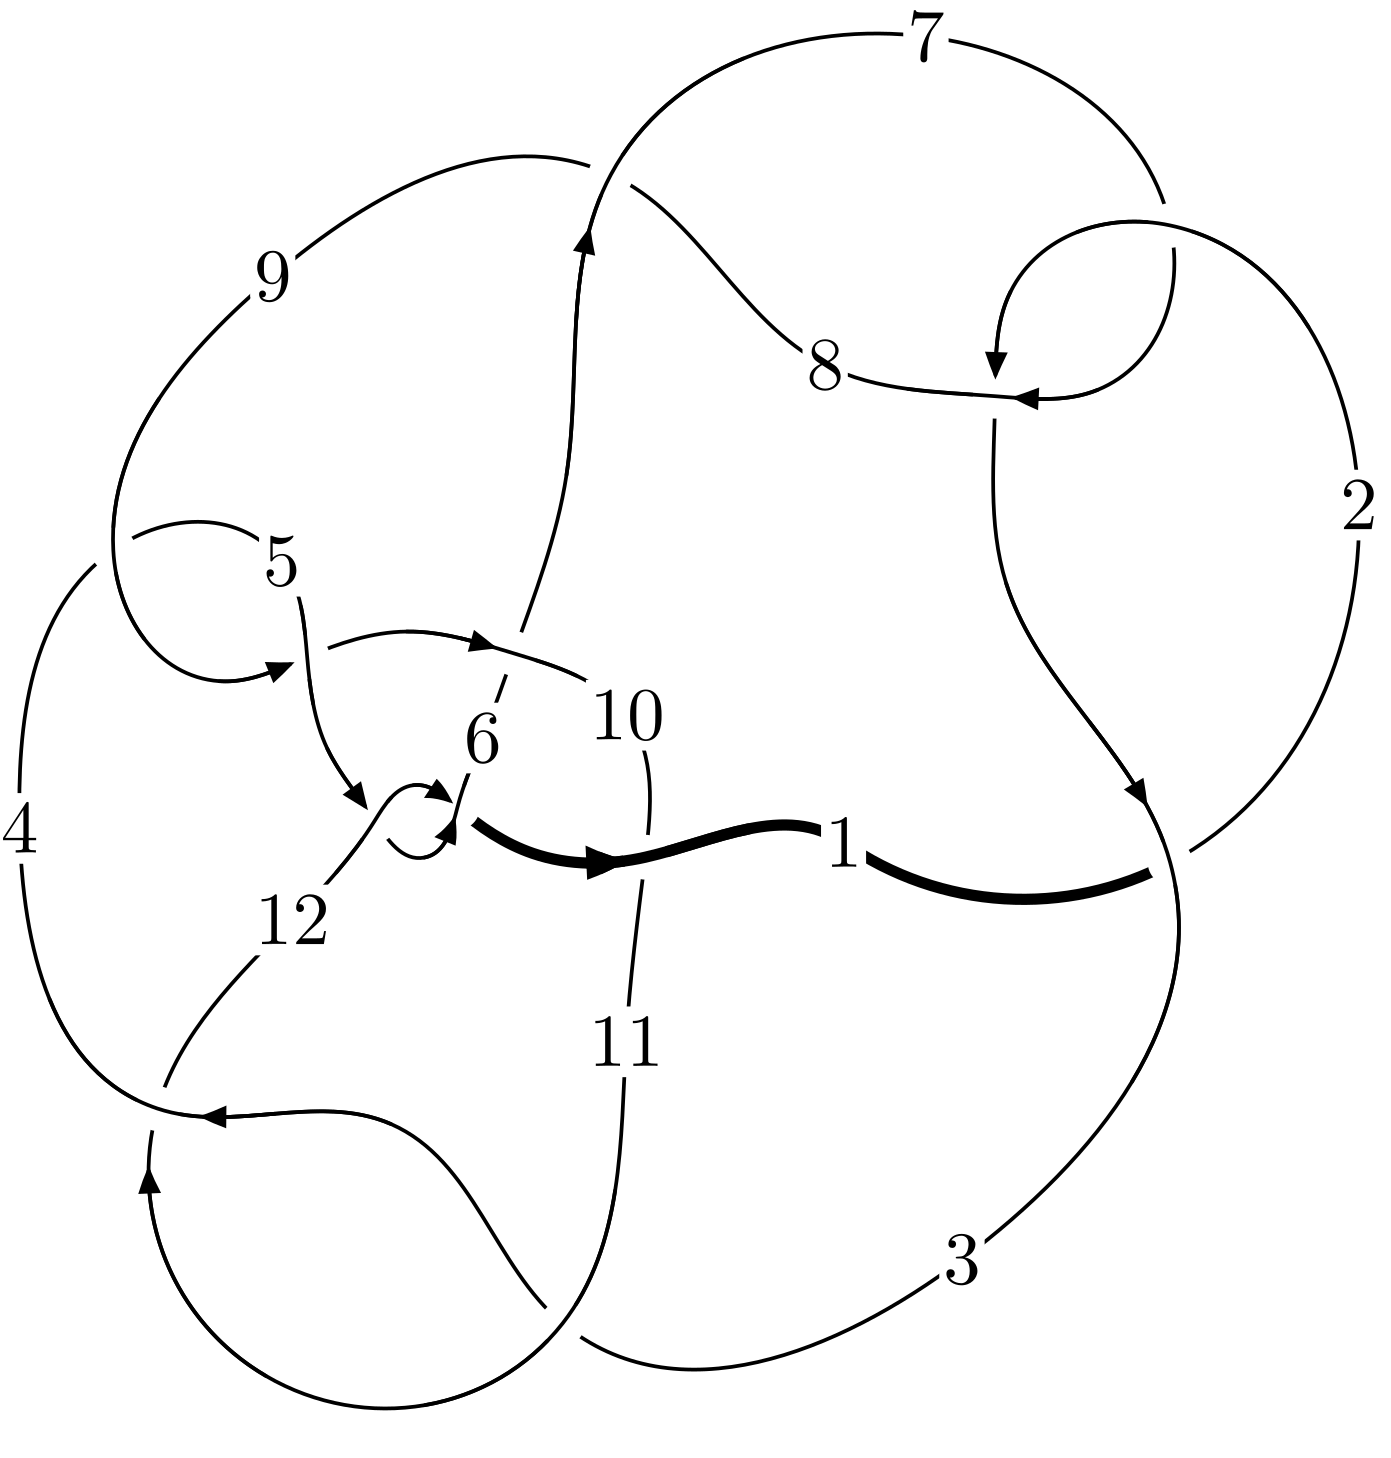
\includegraphics[width=112pt]{../../../GIT/diagram.site/Diagrams/png/1585_12a_0784.png}\\
\ \ \ A knot diagram\footnotemark}&
\allowdisplaybreaks
\textbf{Linearized knot diagam} \\
\cline{2-2}
 &
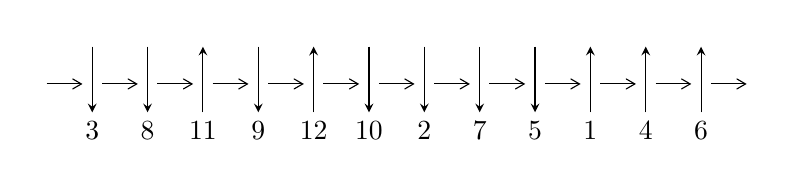
\begin{tikzpicture}[x=20pt, y=17pt]
	% nodes
	\node (C0) at (0, 0) {};
	\node (C1) at (1, 0) {};
	\node (C1U) at (1, +1) {};
	\node (C1D) at (1, -1) {3};

	\node (C2) at (2, 0) {};
	\node (C2U) at (2, +1) {};
	\node (C2D) at (2, -1) {8};

	\node (C3) at (3, 0) {};
	\node (C3U) at (3, +1) {};
	\node (C3D) at (3, -1) {11};

	\node (C4) at (4, 0) {};
	\node (C4U) at (4, +1) {};
	\node (C4D) at (4, -1) {9};

	\node (C5) at (5, 0) {};
	\node (C5U) at (5, +1) {};
	\node (C5D) at (5, -1) {12};

	\node (C6) at (6, 0) {};
	\node (C6U) at (6, +1) {};
	\node (C6D) at (6, -1) {10};

	\node (C7) at (7, 0) {};
	\node (C7U) at (7, +1) {};
	\node (C7D) at (7, -1) {2};

	\node (C8) at (8, 0) {};
	\node (C8U) at (8, +1) {};
	\node (C8D) at (8, -1) {7};

	\node (C9) at (9, 0) {};
	\node (C9U) at (9, +1) {};
	\node (C9D) at (9, -1) {5};

	\node (C10) at (10, 0) {};
	\node (C10U) at (10, +1) {};
	\node (C10D) at (10, -1) {1};

	\node (C11) at (11, 0) {};
	\node (C11U) at (11, +1) {};
	\node (C11D) at (11, -1) {4};

	\node (C12) at (12, 0) {};
	\node (C12U) at (12, +1) {};
	\node (C12D) at (12, -1) {6};
	\node (C13) at (13, 0) {};

	% arrows
	\draw[->,>={angle 60}]
	(C0) edge (C1) (C1) edge (C2) (C2) edge (C3) (C3) edge (C4) (C4) edge (C5) (C5) edge (C6) (C6) edge (C7) (C7) edge (C8) (C8) edge (C9) (C9) edge (C10) (C10) edge (C11) (C11) edge (C12) (C12) edge (C13) ;	\draw[->,>=stealth]
	(C1U) edge (C1D) (C2U) edge (C2D) (C3D) edge (C3U) (C4U) edge (C4D) (C5D) edge (C5U) (C6U) edge (C6D) (C7U) edge (C7D) (C8U) edge (C8D) (C9U) edge (C9D) (C10D) edge (C10U) (C11D) edge (C11U) (C12D) edge (C12U) ;
	\end{tikzpicture} \\
\hhline{~~} \\& 
\textbf{Solving Sequence} \\ \cline{2-2} 
 &
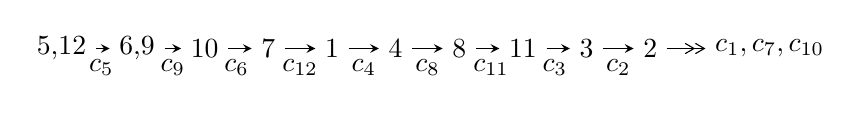
\begin{tikzpicture}[x=23pt, y=7pt]
	% node
	\node (A0) at (-1/8, 0) {5,12};
	\node (A1) at (17/16, 0) {6,9};
	\node (A2) at (17/8, 0) {10};
	\node (A3) at (25/8, 0) {7};
	\node (A4) at (33/8, 0) {1};
	\node (A5) at (41/8, 0) {4};
	\node (A6) at (49/8, 0) {8};
	\node (A7) at (57/8, 0) {11};
	\node (A8) at (65/8, 0) {3};
	\node (A9) at (73/8, 0) {2};
	\node (C1) at (1/2, -1) {$c_{5}$};
	\node (C2) at (13/8, -1) {$c_{9}$};
	\node (C3) at (21/8, -1) {$c_{6}$};
	\node (C4) at (29/8, -1) {$c_{12}$};
	\node (C5) at (37/8, -1) {$c_{4}$};
	\node (C6) at (45/8, -1) {$c_{8}$};
	\node (C7) at (53/8, -1) {$c_{11}$};
	\node (C8) at (61/8, -1) {$c_{3}$};
	\node (C9) at (69/8, -1) {$c_{2}$};
	\node (A10) at (11, 0) {$c_{1},c_{7},c_{10}$};

	% edge
	\draw[->,>=stealth]	
	(A0) edge (A1) (A1) edge (A2) (A2) edge (A3) (A3) edge (A4) (A4) edge (A5) (A5) edge (A6) (A6) edge (A7) (A7) edge (A8) (A8) edge (A9) ;
	\draw[->>,>={angle 60}]	
	(A9) edge (A10);
\end{tikzpicture} \\ 

\end{tabular} \\

\footnotetext{
The image of knot diagram is generated by the software ``\textbf{Draw programme}" developed by Andrew Bartholomew(\url{http://www.layer8.co.uk/maths/draw/index.htm\#Running-draw}), where we modified some parts for our purpose(\url{https://github.com/CATsTAILs/LinksPainter}).
}\phantom \\ \newline 
\centering \textbf{Ideals for irreducible components\footnotemark of $X_{\text{par}}$} 
 
\begin{align*}
I^u_{1}&=\langle 
2.63739\times10^{482} u^{126}+1.73298\times10^{482} u^{125}+\cdots+2.05419\times10^{482} b-2.00818\times10^{485},\\
\phantom{I^u_{1}}&\phantom{= \langle  }-1.32661\times10^{485} u^{126}-1.40289\times10^{485} u^{125}+\cdots+2.36848\times10^{485} a+1.00544\times10^{488},\\
\phantom{I^u_{1}}&\phantom{= \langle  }u^{127}+u^{126}+\cdots-6672 u-1153\rangle \\
I^u_{2}&=\langle 
-286200551 u^{28}-494699359 u^{27}+\cdots+112090025 b+67634672,\\
\phantom{I^u_{2}}&\phantom{= \langle  }-816612824 u^{28}-1336630466 u^{27}+\cdots+112090025 a+558878203,\;u^{29}+u^{28}+\cdots- u+1\rangle \\
I^u_{3}&=\langle 
b- u+1,\;a,\;u^2- u-1\rangle \\
\\
\end{align*}
\raggedright * 3 irreducible components of $\dim_{\mathbb{C}}=0$, with total 158 representations.\\
\footnotetext{All coefficients of polynomials are rational numbers. But the coefficients are sometimes approximated in decimal forms when there is not enough margin.}
\newpage
\renewcommand{\arraystretch}{1}
\centering \section*{I. $I^u_{1}= \langle 2.64\times10^{482} u^{126}+1.73\times10^{482} u^{125}+\cdots+2.05\times10^{482} b-2.01\times10^{485},\;-1.33\times10^{485} u^{126}-1.40\times10^{485} u^{125}+\cdots+2.37\times10^{485} a+1.01\times10^{488},\;u^{127}+u^{126}+\cdots-6672 u-1153 \rangle$}
\flushleft \textbf{(i) Arc colorings}\\
\begin{tabular}{m{7pt} m{180pt} m{7pt} m{180pt} }
\flushright $a_{5}=$&$\begin{pmatrix}1\\0\end{pmatrix}$ \\
\flushright $a_{12}=$&$\begin{pmatrix}0\\u\end{pmatrix}$ \\
\flushright $a_{6}=$&$\begin{pmatrix}1\\- u^2\end{pmatrix}$ \\
\flushright $a_{9}=$&$\begin{pmatrix}0.560111 u^{126}+0.592315 u^{125}+\cdots-752.208 u-424.508\\-1.28391 u^{126}-0.843635 u^{125}+\cdots+3591.97 u+977.602\end{pmatrix}$ \\
\flushright $a_{10}=$&$\begin{pmatrix}1.84402 u^{126}+1.43595 u^{125}+\cdots-4344.18 u-1402.11\\-1.28391 u^{126}-0.843635 u^{125}+\cdots+3591.97 u+977.602\end{pmatrix}$ \\
\flushright $a_{7}=$&$\begin{pmatrix}-0.934886 u^{126}-0.344702 u^{125}+\cdots+5811.23 u+1302.90\\-0.433227 u^{126}+0.455790 u^{125}+\cdots+8089.02 u+1593.55\end{pmatrix}$ \\
\flushright $a_{1}=$&$\begin{pmatrix}u\\- u^3+u\end{pmatrix}$ \\
\flushright $a_{4}=$&$\begin{pmatrix}-0.0709417 u^{126}-0.649720 u^{125}+\cdots-6676.29 u-1248.62\\2.42115 u^{126}+0.505784 u^{125}+\cdots-14133.4 u-3134.64\end{pmatrix}$ \\
\flushright $a_{8}=$&$\begin{pmatrix}-0.0120408 u^{126}+0.123095 u^{125}+\cdots+4476.63 u+997.946\\1.42633 u^{126}-0.415950 u^{125}+\cdots-13110.2 u-2621.56\end{pmatrix}$ \\
\flushright $a_{11}=$&$\begin{pmatrix}0.546467 u^{126}+0.457767 u^{125}+\cdots-1204.38 u-453.814\\-1.74298 u^{126}-1.01022 u^{125}+\cdots+6097.02 u+1557.66\end{pmatrix}$ \\
\flushright $a_{3}=$&$\begin{pmatrix}1.03181 u^{126}+0.0803714 u^{125}+\cdots-7342.95 u-1545.08\\1.99899 u^{126}+0.207011 u^{125}+\cdots-13754.8 u-2953.24\end{pmatrix}$ \\
\flushright $a_{2}=$&$\begin{pmatrix}0.601134 u^{126}-0.502581 u^{125}+\cdots-4109.22 u-598.688\\3.57670 u^{126}+0.360615 u^{125}+\cdots-21584.6 u-4600.97\end{pmatrix}$\\&\end{tabular}
\flushleft \textbf{(ii) Obstruction class $= -1$}\\~\\
\flushleft \textbf{(iii) Cusp Shapes $= -5.36102 u^{126}-0.802747 u^{125}+\cdots+30637.4 u+6600.82$}\\~\\
\newpage\renewcommand{\arraystretch}{1}
\flushleft \textbf{(iv) u-Polynomials at the component}\newline \\
\begin{tabular}{m{50pt}|m{274pt}}
Crossings & \hspace{64pt}u-Polynomials at each crossing \\
\hline $$\begin{aligned}c_{1},c_{8}\end{aligned}$$&$\begin{aligned}
&u^{127}+39 u^{126}+\cdots+1944 u+81
\end{aligned}$\\
\hline $$\begin{aligned}c_{2},c_{7}\end{aligned}$$&$\begin{aligned}
&u^{127}+u^{126}+\cdots+18 u-9
\end{aligned}$\\
\hline $$\begin{aligned}c_{3},c_{11}\end{aligned}$$&$\begin{aligned}
&u^{127}-2 u^{126}+\cdots-91249 u+90319
\end{aligned}$\\
\hline $$\begin{aligned}c_{4},c_{9}\end{aligned}$$&$\begin{aligned}
&u^{127}+2 u^{126}+\cdots-15 u-1
\end{aligned}$\\
\hline $$\begin{aligned}c_{5},c_{12}\end{aligned}$$&$\begin{aligned}
&u^{127}+u^{126}+\cdots-6672 u-1153
\end{aligned}$\\
\hline $$\begin{aligned}c_{6}\end{aligned}$$&$\begin{aligned}
&u^{127}-2 u^{126}+\cdots-934469 u+281173
\end{aligned}$\\
\hline $$\begin{aligned}c_{10}\end{aligned}$$&$\begin{aligned}
&u^{127}+6 u^{126}+\cdots+1248715953 u+143741087
\end{aligned}$\\
\hline
\end{tabular}\\~\\
\newpage\renewcommand{\arraystretch}{1}
\flushleft \textbf{(v) Riley Polynomials at the component}\newline \\
\begin{tabular}{m{50pt}|m{274pt}}
Crossings & \hspace{64pt}Riley Polynomials at each crossing \\
\hline $$\begin{aligned}c_{1},c_{8}\end{aligned}$$&$\begin{aligned}
&y^{127}+109 y^{126}+\cdots+84564 y-6561
\end{aligned}$\\
\hline $$\begin{aligned}c_{2},c_{7}\end{aligned}$$&$\begin{aligned}
&y^{127}-39 y^{126}+\cdots+1944 y-81
\end{aligned}$\\
\hline $$\begin{aligned}c_{3},c_{11}\end{aligned}$$&$\begin{aligned}
&y^{127}-106 y^{126}+\cdots+204122256495 y-8157521761
\end{aligned}$\\
\hline $$\begin{aligned}c_{4},c_{9}\end{aligned}$$&$\begin{aligned}
&y^{127}-66 y^{126}+\cdots+191 y-1
\end{aligned}$\\
\hline $$\begin{aligned}c_{5},c_{12}\end{aligned}$$&$\begin{aligned}
&y^{127}-83 y^{126}+\cdots+49166786 y-1329409
\end{aligned}$\\
\hline $$\begin{aligned}c_{6}\end{aligned}$$&$\begin{aligned}
&y^{127}+22 y^{126}+\cdots-2134776124149 y-79058255929
\end{aligned}$\\
\hline $$\begin{aligned}c_{10}\end{aligned}$$&$\begin{aligned}
&y^{127}-58 y^{126}+\cdots+427269195188756631 y-20661500091941569
\end{aligned}$\\
\hline
\end{tabular}\\~\\
\newpage\flushleft \textbf{(vi) Complex Volumes and Cusp Shapes}
$$\begin{array}{c|c|c}  
\text{Solutions to }I^u_{1}& \I (\text{vol} + \sqrt{-1}CS) & \text{Cusp shape}\\
 \hline 
\begin{aligned}
u &= \phantom{-}0.899609 + 0.424992 I \\
a &= -1.10629 - 0.94682 I \\
b &= -1.11918 + 0.90820 I\end{aligned}
 & -1.07536 + 5.17840 I & \phantom{-0.000000 } 0 \\ \hline\begin{aligned}
u &= \phantom{-}0.899609 - 0.424992 I \\
a &= -1.10629 + 0.94682 I \\
b &= -1.11918 - 0.90820 I\end{aligned}
 & -1.07536 - 5.17840 I & \phantom{-0.000000 } 0 \\ \hline\begin{aligned}
u &= -0.969383 + 0.217043 I \\
a &= -0.242095 + 0.716577 I \\
b &= -1.108500 - 0.431288 I\end{aligned}
 & -2.20885 - 0.84555 I & \phantom{-0.000000 } 0 \\ \hline\begin{aligned}
u &= -0.969383 - 0.217043 I \\
a &= -0.242095 - 0.716577 I \\
b &= -1.108500 + 0.431288 I\end{aligned}
 & -2.20885 + 0.84555 I & \phantom{-0.000000 } 0 \\ \hline\begin{aligned}
u &= \phantom{-}0.975700 + 0.058998 I \\
a &= -1.50968 - 0.43039 I \\
b &= -1.39756 + 0.26312 I\end{aligned}
 & \phantom{-}1.86265 + 1.12684 I & \phantom{-0.000000 } 0 \\ \hline\begin{aligned}
u &= \phantom{-}0.975700 - 0.058998 I \\
a &= -1.50968 + 0.43039 I \\
b &= -1.39756 - 0.26312 I\end{aligned}
 & \phantom{-}1.86265 - 1.12684 I & \phantom{-0.000000 } 0 \\ \hline\begin{aligned}
u &= -0.833264 + 0.468989 I \\
a &= -0.481761 + 0.814515 I \\
b &= -1.350000 + 0.031703 I\end{aligned}
 & \phantom{-}1.37120 + 3.57194 I & \phantom{-0.000000 } 0 \\ \hline\begin{aligned}
u &= -0.833264 - 0.468989 I \\
a &= -0.481761 - 0.814515 I \\
b &= -1.350000 - 0.031703 I\end{aligned}
 & \phantom{-}1.37120 - 3.57194 I & \phantom{-0.000000 } 0 \\ \hline\begin{aligned}
u &= \phantom{-}0.785879 + 0.517921 I \\
a &= \phantom{-}0.504803 + 0.816321 I \\
b &= \phantom{-}1.361010 + 0.150128 I\end{aligned}
 & \phantom{-}1.55196 + 1.85604 I & \phantom{-0.000000 } 0 \\ \hline\begin{aligned}
u &= \phantom{-}0.785879 - 0.517921 I \\
a &= \phantom{-}0.504803 - 0.816321 I \\
b &= \phantom{-}1.361010 - 0.150128 I\end{aligned}
 & \phantom{-}1.55196 - 1.85604 I & \phantom{-0.000000 } 0\\
 \hline 
 \end{array}$$\newpage$$\begin{array}{c|c|c}  
\text{Solutions to }I^u_{1}& \I (\text{vol} + \sqrt{-1}CS) & \text{Cusp shape}\\
 \hline 
\begin{aligned}
u &= -0.921369\phantom{ +0.000000I} \\
a &= \phantom{-}1.14442\phantom{ +0.000000I} \\
b &= \phantom{-}1.76452\phantom{ +0.000000I}\end{aligned}
 & -3.14048\phantom{ +0.000000I} & \phantom{-0.000000 } 0 \\ \hline\begin{aligned}
u &= \phantom{-}0.941710 + 0.530939 I \\
a &= -1.091830 - 0.862514 I \\
b &= -1.00896 + 1.08502 I\end{aligned}
 & \phantom{-}3.99006 + 8.76786 I & \phantom{-0.000000 } 0 \\ \hline\begin{aligned}
u &= \phantom{-}0.941710 - 0.530939 I \\
a &= -1.091830 + 0.862514 I \\
b &= -1.00896 - 1.08502 I\end{aligned}
 & \phantom{-}3.99006 - 8.76786 I & \phantom{-0.000000 } 0 \\ \hline\begin{aligned}
u &= \phantom{-}0.465741 + 0.983160 I \\
a &= \phantom{-}1.42474 - 0.17082 I \\
b &= \phantom{-}1.038660 - 0.084011 I\end{aligned}
 & -3.47260 + 4.47855 I & \phantom{-0.000000 } 0 \\ \hline\begin{aligned}
u &= \phantom{-}0.465741 - 0.983160 I \\
a &= \phantom{-}1.42474 + 0.17082 I \\
b &= \phantom{-}1.038660 + 0.084011 I\end{aligned}
 & -3.47260 - 4.47855 I & \phantom{-0.000000 } 0 \\ \hline\begin{aligned}
u &= \phantom{-}0.910313 + 0.030662 I \\
a &= -0.115819 - 0.906180 I \\
b &= \phantom{-}0.615448 + 0.407124 I\end{aligned}
 & \phantom{-}1.46568 + 0.43178 I & \phantom{-0.000000 } 0 \\ \hline\begin{aligned}
u &= \phantom{-}0.910313 - 0.030662 I \\
a &= -0.115819 + 0.906180 I \\
b &= \phantom{-}0.615448 - 0.407124 I\end{aligned}
 & \phantom{-}1.46568 - 0.43178 I & \phantom{-0.000000 } 0 \\ \hline\begin{aligned}
u &= \phantom{-}0.885847 + 0.205046 I \\
a &= -1.11298 - 0.88899 I \\
b &= -1.33628 + 0.72164 I\end{aligned}
 & \phantom{-}1.31135 + 1.25389 I & \phantom{-0.000000 } 0 \\ \hline\begin{aligned}
u &= \phantom{-}0.885847 - 0.205046 I \\
a &= -1.11298 + 0.88899 I \\
b &= -1.33628 - 0.72164 I\end{aligned}
 & \phantom{-}1.31135 - 1.25389 I & \phantom{-0.000000 } 0 \\ \hline\begin{aligned}
u &= \phantom{-}1.086360 + 0.116517 I \\
a &= \phantom{-}0.035013 + 0.516038 I \\
b &= \phantom{-}0.885902 - 0.829996 I\end{aligned}
 & \phantom{-}2.98971 + 0.94847 I & \phantom{-0.000000 } 0\\
 \hline 
 \end{array}$$\newpage$$\begin{array}{c|c|c}  
\text{Solutions to }I^u_{1}& \I (\text{vol} + \sqrt{-1}CS) & \text{Cusp shape}\\
 \hline 
\begin{aligned}
u &= \phantom{-}1.086360 - 0.116517 I \\
a &= \phantom{-}0.035013 - 0.516038 I \\
b &= \phantom{-}0.885902 + 0.829996 I\end{aligned}
 & \phantom{-}2.98971 - 0.94847 I & \phantom{-0.000000 } 0 \\ \hline\begin{aligned}
u &= -1.066830 + 0.244598 I \\
a &= \phantom{-}1.21273 - 1.16451 I \\
b &= \phantom{-}1.105170 + 0.598534 I\end{aligned}
 & \phantom{-}1.54996 - 5.14937 I & \phantom{-0.000000 } 0 \\ \hline\begin{aligned}
u &= -1.066830 - 0.244598 I \\
a &= \phantom{-}1.21273 + 1.16451 I \\
b &= \phantom{-}1.105170 - 0.598534 I\end{aligned}
 & \phantom{-}1.54996 + 5.14937 I & \phantom{-0.000000 } 0 \\ \hline\begin{aligned}
u &= -0.898348 + 0.070569 I \\
a &= \phantom{-}1.075500 - 0.494864 I \\
b &= \phantom{-}1.65418 + 0.50089 I\end{aligned}
 & \phantom{-}0.62635 - 5.91693 I & \phantom{-0.000000 } 0 \\ \hline\begin{aligned}
u &= -0.898348 - 0.070569 I \\
a &= \phantom{-}1.075500 + 0.494864 I \\
b &= \phantom{-}1.65418 - 0.50089 I\end{aligned}
 & \phantom{-}0.62635 + 5.91693 I & \phantom{-0.000000 } 0 \\ \hline\begin{aligned}
u &= -0.965308 + 0.528116 I \\
a &= \phantom{-}1.070340 - 0.856967 I \\
b &= \phantom{-}0.95027 + 1.08029 I\end{aligned}
 & \phantom{-}4.24976 - 3.00059 I & \phantom{-0.000000 } 0 \\ \hline\begin{aligned}
u &= -0.965308 - 0.528116 I \\
a &= \phantom{-}1.070340 + 0.856967 I \\
b &= \phantom{-}0.95027 - 1.08029 I\end{aligned}
 & \phantom{-}4.24976 + 3.00059 I & \phantom{-0.000000 } 0 \\ \hline\begin{aligned}
u &= -1.090420 + 0.156147 I \\
a &= -0.131377 + 0.486924 I \\
b &= -1.074270 - 0.867636 I\end{aligned}
 & \phantom{-}2.02042 - 6.23432 I & \phantom{-0.000000 } 0 \\ \hline\begin{aligned}
u &= -1.090420 - 0.156147 I \\
a &= -0.131377 - 0.486924 I \\
b &= -1.074270 + 0.867636 I\end{aligned}
 & \phantom{-}2.02042 + 6.23432 I & \phantom{-0.000000 } 0 \\ \hline\begin{aligned}
u &= \phantom{-}1.106460 + 0.094367 I \\
a &= -1.97773 - 1.38977 I \\
b &= -0.993385 + 0.393640 I\end{aligned}
 & \phantom{-}8.69249 + 0.96192 I & \phantom{-0.000000 } 0\\
 \hline 
 \end{array}$$\newpage$$\begin{array}{c|c|c}  
\text{Solutions to }I^u_{1}& \I (\text{vol} + \sqrt{-1}CS) & \text{Cusp shape}\\
 \hline 
\begin{aligned}
u &= \phantom{-}1.106460 - 0.094367 I \\
a &= -1.97773 + 1.38977 I \\
b &= -0.993385 - 0.393640 I\end{aligned}
 & \phantom{-}8.69249 - 0.96192 I & \phantom{-0.000000 } 0 \\ \hline\begin{aligned}
u &= \phantom{-}1.071220 + 0.326687 I \\
a &= -0.670886 - 0.787907 I \\
b &= \phantom{-}0.118526 + 0.756860 I\end{aligned}
 & \phantom{-}6.62998 + 0.44766 I & \phantom{-0.000000 } 0 \\ \hline\begin{aligned}
u &= \phantom{-}1.071220 - 0.326687 I \\
a &= -0.670886 + 0.787907 I \\
b &= \phantom{-}0.118526 - 0.756860 I\end{aligned}
 & \phantom{-}6.62998 - 0.44766 I & \phantom{-0.000000 } 0 \\ \hline\begin{aligned}
u &= -1.117830 + 0.106521 I \\
a &= \phantom{-}1.85098 - 1.49346 I \\
b &= \phantom{-}0.986138 + 0.434205 I\end{aligned}
 & \phantom{-}8.52486 - 7.18622 I & \phantom{-0.000000 } 0 \\ \hline\begin{aligned}
u &= -1.117830 - 0.106521 I \\
a &= \phantom{-}1.85098 + 1.49346 I \\
b &= \phantom{-}0.986138 - 0.434205 I\end{aligned}
 & \phantom{-}8.52486 + 7.18622 I & \phantom{-0.000000 } 0 \\ \hline\begin{aligned}
u &= \phantom{-}0.534383 + 0.689920 I \\
a &= \phantom{-}0.478682 + 0.686201 I \\
b &= \phantom{-}1.160460 + 0.697958 I\end{aligned}
 & \phantom{-}2.82278 - 4.08425 I & \phantom{-0.000000 } 0 \\ \hline\begin{aligned}
u &= \phantom{-}0.534383 - 0.689920 I \\
a &= \phantom{-}0.478682 - 0.686201 I \\
b &= \phantom{-}1.160460 - 0.697958 I\end{aligned}
 & \phantom{-}2.82278 + 4.08425 I & \phantom{-0.000000 } 0 \\ \hline\begin{aligned}
u &= -1.067680 + 0.371245 I \\
a &= \phantom{-}0.733164 - 0.800903 I \\
b &= -0.003651 + 0.784977 I\end{aligned}
 & \phantom{-}6.42520 - 6.45218 I & \phantom{-0.000000 } 0 \\ \hline\begin{aligned}
u &= -1.067680 - 0.371245 I \\
a &= \phantom{-}0.733164 + 0.800903 I \\
b &= -0.003651 - 0.784977 I\end{aligned}
 & \phantom{-}6.42520 + 6.45218 I & \phantom{-0.000000 } 0 \\ \hline\begin{aligned}
u &= \phantom{-}0.620487 + 0.589256 I \\
a &= \phantom{-}0.548489 + 0.759148 I \\
b &= \phantom{-}1.217960 + 0.436850 I\end{aligned}
 & -1.83228 - 1.08155 I & \phantom{-0.000000 } 0\\
 \hline 
 \end{array}$$\newpage$$\begin{array}{c|c|c}  
\text{Solutions to }I^u_{1}& \I (\text{vol} + \sqrt{-1}CS) & \text{Cusp shape}\\
 \hline 
\begin{aligned}
u &= \phantom{-}0.620487 - 0.589256 I \\
a &= \phantom{-}0.548489 - 0.759148 I \\
b &= \phantom{-}1.217960 - 0.436850 I\end{aligned}
 & -1.83228 + 1.08155 I & \phantom{-0.000000 } 0 \\ \hline\begin{aligned}
u &= -1.045130 + 0.469194 I \\
a &= \phantom{-}0.946605 - 0.934179 I \\
b &= \phantom{-}0.788954 + 0.736081 I\end{aligned}
 & \phantom{-}0.47688 - 4.49237 I & \phantom{-0.000000 } 0 \\ \hline\begin{aligned}
u &= -1.045130 - 0.469194 I \\
a &= \phantom{-}0.946605 + 0.934179 I \\
b &= \phantom{-}0.788954 - 0.736081 I\end{aligned}
 & \phantom{-}0.47688 + 4.49237 I & \phantom{-0.000000 } 0 \\ \hline\begin{aligned}
u &= -0.502135 + 0.687224 I \\
a &= -0.472241 + 0.657894 I \\
b &= -1.092990 + 0.722258 I\end{aligned}
 & \phantom{-}2.92596 - 1.65726 I & \phantom{-0.000000 } 0 \\ \hline\begin{aligned}
u &= -0.502135 - 0.687224 I \\
a &= -0.472241 - 0.657894 I \\
b &= -1.092990 - 0.722258 I\end{aligned}
 & \phantom{-}2.92596 + 1.65726 I & \phantom{-0.000000 } 0 \\ \hline\begin{aligned}
u &= -0.435982 + 0.722667 I \\
a &= -1.396900 - 0.103093 I \\
b &= -0.943841 + 0.061516 I\end{aligned}
 & -1.65126 + 0.13326 I & \phantom{-0.000000 } 0 \\ \hline\begin{aligned}
u &= -0.435982 - 0.722667 I \\
a &= -1.396900 + 0.103093 I \\
b &= -0.943841 - 0.061516 I\end{aligned}
 & -1.65126 - 0.13326 I & \phantom{-0.000000 } 0 \\ \hline\begin{aligned}
u &= \phantom{-}0.256758 + 0.792899 I \\
a &= -1.52637 - 0.60838 I \\
b &= -0.400374 - 0.677480 I\end{aligned}
 & \phantom{-}7.42361 + 0.98363 I & \phantom{-0.000000 } 0 \\ \hline\begin{aligned}
u &= \phantom{-}0.256758 - 0.792899 I \\
a &= -1.52637 + 0.60838 I \\
b &= -0.400374 + 0.677480 I\end{aligned}
 & \phantom{-}7.42361 - 0.98363 I & \phantom{-0.000000 } 0 \\ \hline\begin{aligned}
u &= \phantom{-}0.158435 + 0.811000 I \\
a &= \phantom{-}1.58987 - 0.20219 I \\
b &= \phantom{-}1.186190 + 0.129187 I\end{aligned}
 & -5.85707 - 1.88338 I & \phantom{-0.000000 } 0\\
 \hline 
 \end{array}$$\newpage$$\begin{array}{c|c|c}  
\text{Solutions to }I^u_{1}& \I (\text{vol} + \sqrt{-1}CS) & \text{Cusp shape}\\
 \hline 
\begin{aligned}
u &= \phantom{-}0.158435 - 0.811000 I \\
a &= \phantom{-}1.58987 + 0.20219 I \\
b &= \phantom{-}1.186190 - 0.129187 I\end{aligned}
 & -5.85707 + 1.88338 I & \phantom{-0.000000 } 0 \\ \hline\begin{aligned}
u &= \phantom{-}0.110570 + 1.195880 I \\
a &= -1.335490 - 0.397774 I \\
b &= -1.073010 - 0.594550 I\end{aligned}
 & \phantom{-}5.53142 - 5.95429 I & \phantom{-0.000000 } 0 \\ \hline\begin{aligned}
u &= \phantom{-}0.110570 - 1.195880 I \\
a &= -1.335490 + 0.397774 I \\
b &= -1.073010 + 0.594550 I\end{aligned}
 & \phantom{-}5.53142 + 5.95429 I & \phantom{-0.000000 } 0 \\ \hline\begin{aligned}
u &= -0.089749 + 1.201270 I \\
a &= \phantom{-}1.339290 - 0.390590 I \\
b &= \phantom{-}1.122270 - 0.584605 I\end{aligned}
 & \phantom{-}4.52673 + 12.24300 I & \phantom{-0.000000 } 0 \\ \hline\begin{aligned}
u &= -0.089749 - 1.201270 I \\
a &= \phantom{-}1.339290 + 0.390590 I \\
b &= \phantom{-}1.122270 + 0.584605 I\end{aligned}
 & \phantom{-}4.52673 - 12.24300 I & \phantom{-0.000000 } 0 \\ \hline\begin{aligned}
u &= -1.118870 + 0.449295 I \\
a &= \phantom{-}0.878072 - 1.027960 I \\
b &= \phantom{-}0.920268 + 0.556646 I\end{aligned}
 & \phantom{-}0.54978 - 4.62144 I & \phantom{-0.000000 } 0 \\ \hline\begin{aligned}
u &= -1.118870 - 0.449295 I \\
a &= \phantom{-}0.878072 + 1.027960 I \\
b &= \phantom{-}0.920268 - 0.556646 I\end{aligned}
 & \phantom{-}0.54978 + 4.62144 I & \phantom{-0.000000 } 0 \\ \hline\begin{aligned}
u &= -0.745220 + 0.204465 I \\
a &= \phantom{-}0.07001 - 1.44950 I \\
b &= -0.394495 + 0.100817 I\end{aligned}
 & -0.32061 - 3.50677 I & \phantom{-0.000000 } 0 \\ \hline\begin{aligned}
u &= -0.745220 - 0.204465 I \\
a &= \phantom{-}0.07001 + 1.44950 I \\
b &= -0.394495 - 0.100817 I\end{aligned}
 & -0.32061 + 3.50677 I & \phantom{-0.000000 } 0 \\ \hline\begin{aligned}
u &= -0.728800 + 0.172451 I \\
a &= \phantom{-}1.41642 - 2.53956 I \\
b &= -0.269398 - 0.042175 I\end{aligned}
 & \phantom{-}6.73042 - 6.79692 I & \phantom{-0.000000 } 0\\
 \hline 
 \end{array}$$\newpage$$\begin{array}{c|c|c}  
\text{Solutions to }I^u_{1}& \I (\text{vol} + \sqrt{-1}CS) & \text{Cusp shape}\\
 \hline 
\begin{aligned}
u &= -0.728800 - 0.172451 I \\
a &= \phantom{-}1.41642 + 2.53956 I \\
b &= -0.269398 + 0.042175 I\end{aligned}
 & \phantom{-}6.73042 + 6.79692 I & \phantom{-0.000000 } 0 \\ \hline\begin{aligned}
u &= -0.223887 + 0.712552 I \\
a &= \phantom{-}1.63558 - 0.63068 I \\
b &= \phantom{-}0.283171 - 0.714554 I\end{aligned}
 & \phantom{-}6.85744 - 7.23141 I & \phantom{-0.000000 } 0 \\ \hline\begin{aligned}
u &= -0.223887 - 0.712552 I \\
a &= \phantom{-}1.63558 + 0.63068 I \\
b &= \phantom{-}0.283171 + 0.714554 I\end{aligned}
 & \phantom{-}6.85744 + 7.23141 I & \phantom{-0.000000 } 0 \\ \hline\begin{aligned}
u &= \phantom{-}0.315325 + 1.215630 I \\
a &= -1.272500 - 0.456206 I \\
b &= -0.851784 - 0.462480 I\end{aligned}
 & \phantom{-}1.67897 - 1.92022 I & \phantom{-0.000000 } 0 \\ \hline\begin{aligned}
u &= \phantom{-}0.315325 - 1.215630 I \\
a &= -1.272500 + 0.456206 I \\
b &= -0.851784 + 0.462480 I\end{aligned}
 & \phantom{-}1.67897 + 1.92022 I & \phantom{-0.000000 } 0 \\ \hline\begin{aligned}
u &= \phantom{-}0.713232 + 0.155152 I \\
a &= -1.72331 - 2.33254 I \\
b &= \phantom{-}0.267307 - 0.045218 I\end{aligned}
 & \phantom{-}7.03336 + 0.58707 I & \phantom{-0.000000 } 0 \\ \hline\begin{aligned}
u &= \phantom{-}0.713232 - 0.155152 I \\
a &= -1.72331 + 2.33254 I \\
b &= \phantom{-}0.267307 + 0.045218 I\end{aligned}
 & \phantom{-}7.03336 - 0.58707 I & \phantom{-0.000000 } 0 \\ \hline\begin{aligned}
u &= \phantom{-}1.284030 + 0.310582 I \\
a &= -0.0338741 + 0.0205357 I \\
b &= -0.258211 - 1.200890 I\end{aligned}
 & \phantom{-}4.42676 + 6.00018 I & \phantom{-0.000000 } 0 \\ \hline\begin{aligned}
u &= \phantom{-}1.284030 - 0.310582 I \\
a &= -0.0338741 - 0.0205357 I \\
b &= -0.258211 + 1.200890 I\end{aligned}
 & \phantom{-}4.42676 - 6.00018 I & \phantom{-0.000000 } 0 \\ \hline\begin{aligned}
u &= -0.030399 + 0.678002 I \\
a &= \phantom{-}1.82967 - 0.36505 I \\
b &= \phantom{-}1.264820 + 0.355903 I\end{aligned}
 & -0.64284 - 7.09594 I & -5.07346 + 6.77744 I\\
 \hline 
 \end{array}$$\newpage$$\begin{array}{c|c|c}  
\text{Solutions to }I^u_{1}& \I (\text{vol} + \sqrt{-1}CS) & \text{Cusp shape}\\
 \hline 
\begin{aligned}
u &= -0.030399 - 0.678002 I \\
a &= \phantom{-}1.82967 + 0.36505 I \\
b &= \phantom{-}1.264820 - 0.355903 I\end{aligned}
 & -0.64284 + 7.09594 I & -5.07346 - 6.77744 I \\ \hline\begin{aligned}
u &= \phantom{-}1.175060 + 0.609769 I \\
a &= -0.762664 - 0.880020 I \\
b &= -0.872464 + 0.252078 I\end{aligned}
 & -1.06435 + 1.29725 I & \phantom{-0.000000 } 0 \\ \hline\begin{aligned}
u &= \phantom{-}1.175060 - 0.609769 I \\
a &= -0.762664 + 0.880020 I \\
b &= -0.872464 - 0.252078 I\end{aligned}
 & -1.06435 - 1.29725 I & \phantom{-0.000000 } 0 \\ \hline\begin{aligned}
u &= -1.272320 + 0.367407 I \\
a &= \phantom{-}0.68412 - 1.26924 I \\
b &= \phantom{-}1.135280 + 0.549511 I\end{aligned}
 & \phantom{-}3.93987 - 5.23803 I & \phantom{-0.000000 } 0 \\ \hline\begin{aligned}
u &= -1.272320 - 0.367407 I \\
a &= \phantom{-}0.68412 + 1.26924 I \\
b &= \phantom{-}1.135280 - 0.549511 I\end{aligned}
 & \phantom{-}3.93987 + 5.23803 I & \phantom{-0.000000 } 0 \\ \hline\begin{aligned}
u &= \phantom{-}1.269610 + 0.394723 I \\
a &= \phantom{-}0.0409520 - 0.0525356 I \\
b &= -0.50725 - 1.32126 I\end{aligned}
 & \phantom{-}11.1187 + 11.2500 I & \phantom{-0.000000 } 0 \\ \hline\begin{aligned}
u &= \phantom{-}1.269610 - 0.394723 I \\
a &= \phantom{-}0.0409520 + 0.0525356 I \\
b &= -0.50725 + 1.32126 I\end{aligned}
 & \phantom{-}11.1187 - 11.2500 I & \phantom{-0.000000 } 0 \\ \hline\begin{aligned}
u &= -0.427878 + 0.513104 I \\
a &= -0.835560 + 0.459521 I \\
b &= -0.854553 + 0.377787 I\end{aligned}
 & -1.286080 + 0.455261 I & -7.70736 + 1.32907 I \\ \hline\begin{aligned}
u &= -0.427878 - 0.513104 I \\
a &= -0.835560 - 0.459521 I \\
b &= -0.854553 - 0.377787 I\end{aligned}
 & -1.286080 - 0.455261 I & -7.70736 - 1.32907 I \\ \hline\begin{aligned}
u &= \phantom{-}1.250100 + 0.466607 I \\
a &= -0.683965 - 1.073830 I \\
b &= -1.075790 + 0.420354 I\end{aligned}
 & -2.44640 + 6.61908 I & \phantom{-0.000000 } 0\\
 \hline 
 \end{array}$$\newpage$$\begin{array}{c|c|c}  
\text{Solutions to }I^u_{1}& \I (\text{vol} + \sqrt{-1}CS) & \text{Cusp shape}\\
 \hline 
\begin{aligned}
u &= \phantom{-}1.250100 - 0.466607 I \\
a &= -0.683965 + 1.073830 I \\
b &= -1.075790 - 0.420354 I\end{aligned}
 & -2.44640 - 6.61908 I & \phantom{-0.000000 } 0 \\ \hline\begin{aligned}
u &= -0.158795 + 1.330380 I \\
a &= \phantom{-}1.283370 - 0.378700 I \\
b &= \phantom{-}1.006120 - 0.419750 I\end{aligned}
 & -2.71266 + 5.78701 I & \phantom{-0.000000 } 0 \\ \hline\begin{aligned}
u &= -0.158795 - 1.330380 I \\
a &= \phantom{-}1.283370 + 0.378700 I \\
b &= \phantom{-}1.006120 + 0.419750 I\end{aligned}
 & -2.71266 - 5.78701 I & \phantom{-0.000000 } 0 \\ \hline\begin{aligned}
u &= \phantom{-}1.290630 + 0.383162 I \\
a &= -0.637761 - 1.244490 I \\
b &= -1.159890 + 0.528856 I\end{aligned}
 & \phantom{-}3.39980 + 11.12530 I & \phantom{-0.000000 } 0 \\ \hline\begin{aligned}
u &= \phantom{-}1.290630 - 0.383162 I \\
a &= -0.637761 + 1.244490 I \\
b &= -1.159890 - 0.528856 I\end{aligned}
 & \phantom{-}3.39980 - 11.12530 I & \phantom{-0.000000 } 0 \\ \hline\begin{aligned}
u &= -1.289890 + 0.395097 I \\
a &= -0.0207285 - 0.0679971 I \\
b &= \phantom{-}0.524654 - 1.259980 I\end{aligned}
 & \phantom{-}11.90370 - 5.14638 I & \phantom{-0.000000 } 0 \\ \hline\begin{aligned}
u &= -1.289890 - 0.395097 I \\
a &= -0.0207285 + 0.0679971 I \\
b &= \phantom{-}0.524654 + 1.259980 I\end{aligned}
 & \phantom{-}11.90370 + 5.14638 I & \phantom{-0.000000 } 0 \\ \hline\begin{aligned}
u &= -1.217590 + 0.670566 I \\
a &= -1.61163 + 0.39154 I \\
b &= -0.946882 - 0.528758 I\end{aligned}
 & \phantom{-}9.26360 + 1.80665 I & \phantom{-0.000000 } 0 \\ \hline\begin{aligned}
u &= -1.217590 - 0.670566 I \\
a &= -1.61163 - 0.39154 I \\
b &= -0.946882 + 0.528758 I\end{aligned}
 & \phantom{-}9.26360 - 1.80665 I & \phantom{-0.000000 } 0 \\ \hline\begin{aligned}
u &= -0.030368 + 0.608580 I \\
a &= -0.032047 + 0.352615 I \\
b &= -0.059994 + 0.820870 I\end{aligned}
 & \phantom{-}3.49662 + 2.89047 I & -0.32814 - 2.83025 I\\
 \hline 
 \end{array}$$\newpage$$\begin{array}{c|c|c}  
\text{Solutions to }I^u_{1}& \I (\text{vol} + \sqrt{-1}CS) & \text{Cusp shape}\\
 \hline 
\begin{aligned}
u &= -0.030368 - 0.608580 I \\
a &= -0.032047 - 0.352615 I \\
b &= -0.059994 - 0.820870 I\end{aligned}
 & \phantom{-}3.49662 - 2.89047 I & -0.32814 + 2.83025 I \\ \hline\begin{aligned}
u &= -1.368090 + 0.313616 I \\
a &= \phantom{-}0.1135650 - 0.0396663 I \\
b &= \phantom{-}0.356367 - 0.956192 I\end{aligned}
 & \phantom{-}7.68279 - 2.73588 I & \phantom{-0.000000 } 0 \\ \hline\begin{aligned}
u &= -1.368090 - 0.313616 I \\
a &= \phantom{-}0.1135650 + 0.0396663 I \\
b &= \phantom{-}0.356367 + 0.956192 I\end{aligned}
 & \phantom{-}7.68279 + 2.73588 I & \phantom{-0.000000 } 0 \\ \hline\begin{aligned}
u &= \phantom{-}1.397660 + 0.141411 I \\
a &= -0.261924 + 0.078658 I \\
b &= \phantom{-}0.047609 - 0.650115 I\end{aligned}
 & \phantom{-}4.27409 - 0.09782 I & \phantom{-0.000000 } 0 \\ \hline\begin{aligned}
u &= \phantom{-}1.397660 - 0.141411 I \\
a &= -0.261924 - 0.078658 I \\
b &= \phantom{-}0.047609 + 0.650115 I\end{aligned}
 & \phantom{-}4.27409 + 0.09782 I & \phantom{-0.000000 } 0 \\ \hline\begin{aligned}
u &= -0.001739 + 0.590856 I \\
a &= -1.99205 - 0.28236 I \\
b &= -1.178080 + 0.395962 I\end{aligned}
 & \phantom{-}0.06673 + 1.46934 I & -3.77347 - 1.94821 I \\ \hline\begin{aligned}
u &= -0.001739 - 0.590856 I \\
a &= -1.99205 + 0.28236 I \\
b &= -1.178080 - 0.395962 I\end{aligned}
 & \phantom{-}0.06673 - 1.46934 I & -3.77347 + 1.94821 I \\ \hline\begin{aligned}
u &= -0.584488 + 1.282970 I \\
a &= \phantom{-}1.156800 - 0.490604 I \\
b &= \phantom{-}0.794712 - 0.304872 I\end{aligned}
 & -1.74040 - 2.72976 I & \phantom{-0.000000 } 0 \\ \hline\begin{aligned}
u &= -0.584488 - 1.282970 I \\
a &= \phantom{-}1.156800 + 0.490604 I \\
b &= \phantom{-}0.794712 + 0.304872 I\end{aligned}
 & -1.74040 + 2.72976 I & \phantom{-0.000000 } 0 \\ \hline\begin{aligned}
u &= \phantom{-}1.25413 + 0.65584 I \\
a &= \phantom{-}1.56004 + 0.46546 I \\
b &= \phantom{-}0.982720 - 0.572883 I\end{aligned}
 & \phantom{-}10.07250 + 4.68382 I & \phantom{-0.000000 } 0\\
 \hline 
 \end{array}$$\newpage$$\begin{array}{c|c|c}  
\text{Solutions to }I^u_{1}& \I (\text{vol} + \sqrt{-1}CS) & \text{Cusp shape}\\
 \hline 
\begin{aligned}
u &= \phantom{-}1.25413 - 0.65584 I \\
a &= \phantom{-}1.56004 - 0.46546 I \\
b &= \phantom{-}0.982720 + 0.572883 I\end{aligned}
 & \phantom{-}10.07250 - 4.68382 I & \phantom{-0.000000 } 0 \\ \hline\begin{aligned}
u &= \phantom{-}1.43785 + 0.04048 I \\
a &= -0.535512 - 0.137324 I \\
b &= \phantom{-}0.713551 + 0.400227 I\end{aligned}
 & \phantom{-}9.48279 + 3.64685 I & \phantom{-0.000000 } 0 \\ \hline\begin{aligned}
u &= \phantom{-}1.43785 - 0.04048 I \\
a &= -0.535512 + 0.137324 I \\
b &= \phantom{-}0.713551 - 0.400227 I\end{aligned}
 & \phantom{-}9.48279 - 3.64685 I & \phantom{-0.000000 } 0 \\ \hline\begin{aligned}
u &= \phantom{-}0.553209 + 0.067349 I \\
a &= -1.098260 - 0.704150 I \\
b &= \phantom{-}0.358204 - 0.037734 I\end{aligned}
 & \phantom{-}1.291040 + 0.409621 I & \phantom{-}6.92214 - 0.12402 I \\ \hline\begin{aligned}
u &= \phantom{-}0.553209 - 0.067349 I \\
a &= -1.098260 + 0.704150 I \\
b &= \phantom{-}0.358204 + 0.037734 I\end{aligned}
 & \phantom{-}1.291040 - 0.409621 I & \phantom{-}6.92214 + 0.12402 I \\ \hline\begin{aligned}
u &= -1.45221 + 0.03510 I \\
a &= \phantom{-}0.549371 - 0.108937 I \\
b &= -0.751998 + 0.326051 I\end{aligned}
 & \phantom{-}9.62150 + 2.15278 I & \phantom{-0.000000 } 0 \\ \hline\begin{aligned}
u &= -1.45221 - 0.03510 I \\
a &= \phantom{-}0.549371 + 0.108937 I \\
b &= -0.751998 - 0.326051 I\end{aligned}
 & \phantom{-}9.62150 - 2.15278 I & \phantom{-0.000000 } 0 \\ \hline\begin{aligned}
u &= -0.370734 + 0.393926 I \\
a &= -0.429653 - 0.083886 I \\
b &= -0.494247 + 0.281919 I\end{aligned}
 & -1.210000 + 0.364522 I & -7.31156 - 0.42344 I \\ \hline\begin{aligned}
u &= -0.370734 - 0.393926 I \\
a &= -0.429653 + 0.083886 I \\
b &= -0.494247 - 0.281919 I\end{aligned}
 & -1.210000 - 0.364522 I & -7.31156 + 0.42344 I \\ \hline\begin{aligned}
u &= -1.46400\phantom{ +0.000000I} \\
a &= \phantom{-}0.528721\phantom{ +0.000000I} \\
b &= -0.689013\phantom{ +0.000000I}\end{aligned}
 & \phantom{-}5.43041\phantom{ +0.000000I} & \phantom{-0.000000 } 0\\
 \hline 
 \end{array}$$\newpage$$\begin{array}{c|c|c}  
\text{Solutions to }I^u_{1}& \I (\text{vol} + \sqrt{-1}CS) & \text{Cusp shape}\\
 \hline 
\begin{aligned}
u &= \phantom{-}1.36214 + 0.59920 I \\
a &= \phantom{-}1.23814 + 0.71467 I \\
b &= \phantom{-}1.24462 - 0.77204 I\end{aligned}
 & \phantom{-}9.5011 + 12.2560 I & \phantom{-0.000000 } 0 \\ \hline\begin{aligned}
u &= \phantom{-}1.36214 - 0.59920 I \\
a &= \phantom{-}1.23814 - 0.71467 I \\
b &= \phantom{-}1.24462 + 0.77204 I\end{aligned}
 & \phantom{-}9.5011 - 12.2560 I & \phantom{-0.000000 } 0 \\ \hline\begin{aligned}
u &= -1.36570 + 0.59786 I \\
a &= -1.211510 + 0.722450 I \\
b &= -1.27196 - 0.77970 I\end{aligned}
 & \phantom{-}8.5561 - 18.5437 I & \phantom{-0.000000 } 0 \\ \hline\begin{aligned}
u &= -1.36570 - 0.59786 I \\
a &= -1.211510 - 0.722450 I \\
b &= -1.27196 + 0.77970 I\end{aligned}
 & \phantom{-}8.5561 + 18.5437 I & \phantom{-0.000000 } 0 \\ \hline\begin{aligned}
u &= \phantom{-}1.35288 + 0.63179 I \\
a &= \phantom{-}1.30740 + 0.57713 I \\
b &= \phantom{-}1.176410 - 0.646957 I\end{aligned}
 & \phantom{-}5.19449 + 8.54254 I & \phantom{-0.000000 } 0 \\ \hline\begin{aligned}
u &= \phantom{-}1.35288 - 0.63179 I \\
a &= \phantom{-}1.30740 - 0.57713 I \\
b &= \phantom{-}1.176410 + 0.646957 I\end{aligned}
 & \phantom{-}5.19449 - 8.54254 I & \phantom{-0.000000 } 0 \\ \hline\begin{aligned}
u &= -1.37309 + 0.61522 I \\
a &= -1.212770 + 0.607975 I \\
b &= -1.26327 - 0.66728 I\end{aligned}
 & \phantom{-}1.28295 - 12.44340 I & \phantom{-0.000000 } 0 \\ \hline\begin{aligned}
u &= -1.37309 - 0.61522 I \\
a &= -1.212770 - 0.607975 I \\
b &= -1.26327 + 0.66728 I\end{aligned}
 & \phantom{-}1.28295 + 12.44340 I & \phantom{-0.000000 } 0 \\ \hline\begin{aligned}
u &= -1.36625 + 0.67954 I \\
a &= -1.304500 + 0.449717 I \\
b &= -1.166820 - 0.541799 I\end{aligned}
 & \phantom{-}1.26955 - 4.49210 I & \phantom{-0.000000 } 0 \\ \hline\begin{aligned}
u &= -1.36625 - 0.67954 I \\
a &= -1.304500 - 0.449717 I \\
b &= -1.166820 + 0.541799 I\end{aligned}
 & \phantom{-}1.26955 + 4.49210 I & \phantom{-0.000000 } 0\\
 \hline 
 \end{array}$$\newpage$$\begin{array}{c|c|c}  
\text{Solutions to }I^u_{1}& \I (\text{vol} + \sqrt{-1}CS) & \text{Cusp shape}\\
 \hline 
\begin{aligned}
u &= \phantom{-}1.55952\phantom{ +0.000000I} \\
a &= -0.369842\phantom{ +0.000000I} \\
b &= -0.107026\phantom{ +0.000000I}\end{aligned}
 & \phantom{-}4.40346\phantom{ +0.000000I} & \phantom{-0.000000 } 0 \\ \hline\begin{aligned}
u &= -1.53003 + 0.40063 I \\
a &= \phantom{-}0.239958 - 0.198517 I \\
b &= \phantom{-}0.672186 - 0.604197 I\end{aligned}
 & \phantom{-}11.05410 - 0.02645 I & \phantom{-0.000000 } 0 \\ \hline\begin{aligned}
u &= -1.53003 - 0.40063 I \\
a &= \phantom{-}0.239958 + 0.198517 I \\
b &= \phantom{-}0.672186 + 0.604197 I\end{aligned}
 & \phantom{-}11.05410 + 0.02645 I & \phantom{-0.000000 } 0 \\ \hline\begin{aligned}
u &= -0.392255 + 0.133279 I \\
a &= \phantom{-}1.09057 - 2.12779 I \\
b &= -0.415248 - 0.317817 I\end{aligned}
 & -0.33314 - 3.44474 I & -1.95232 + 7.26627 I \\ \hline\begin{aligned}
u &= -0.392255 - 0.133279 I \\
a &= \phantom{-}1.09057 + 2.12779 I \\
b &= -0.415248 + 0.317817 I\end{aligned}
 & -0.33314 + 3.44474 I & -1.95232 - 7.26627 I \\ \hline\begin{aligned}
u &= \phantom{-}1.57828 + 0.43033 I \\
a &= -0.289281 - 0.232214 I \\
b &= -0.729025 - 0.506644 I\end{aligned}
 & \phantom{-}9.98593 - 6.02268 I & \phantom{-0.000000 } 0 \\ \hline\begin{aligned}
u &= \phantom{-}1.57828 - 0.43033 I \\
a &= -0.289281 + 0.232214 I \\
b &= -0.729025 + 0.506644 I\end{aligned}
 & \phantom{-}9.98593 + 6.02268 I & \phantom{-0.000000 } 0\\
 \hline 
 \end{array}$$\newpage\newpage\renewcommand{\arraystretch}{1}
\centering \section*{II. $I^u_{2}= \langle -2.86\times10^{8} u^{28}-4.95\times10^{8} u^{27}+\cdots+1.12\times10^{8} b+6.76\times10^{7},\;-8.17\times10^{8} u^{28}-1.34\times10^{9} u^{27}+\cdots+1.12\times10^{8} a+5.59\times10^{8},\;u^{29}+u^{28}+\cdots- u+1 \rangle$}
\flushleft \textbf{(i) Arc colorings}\\
\begin{tabular}{m{7pt} m{180pt} m{7pt} m{180pt} }
\flushright $a_{5}=$&$\begin{pmatrix}1\\0\end{pmatrix}$ \\
\flushright $a_{12}=$&$\begin{pmatrix}0\\u\end{pmatrix}$ \\
\flushright $a_{6}=$&$\begin{pmatrix}1\\- u^2\end{pmatrix}$ \\
\flushright $a_{9}=$&$\begin{pmatrix}7.28533 u^{28}+11.9246 u^{27}+\cdots+3.04539 u-4.98598\\2.55331 u^{28}+4.41341 u^{27}+\cdots+3.99911 u-0.603396\end{pmatrix}$ \\
\flushright $a_{10}=$&$\begin{pmatrix}4.73202 u^{28}+7.51120 u^{27}+\cdots-0.953725 u-4.38258\\2.55331 u^{28}+4.41341 u^{27}+\cdots+3.99911 u-0.603396\end{pmatrix}$ \\
\flushright $a_{7}=$&$\begin{pmatrix}-2.17231 u^{28}-4.24622 u^{27}+\cdots-0.543133 u+11.1661\\u^{27}+u^{26}+\cdots+2 u^2+u\end{pmatrix}$ \\
\flushright $a_{1}=$&$\begin{pmatrix}u\\- u^3+u\end{pmatrix}$ \\
\flushright $a_{4}=$&$\begin{pmatrix}0.603396 u^{28}+2.15671 u^{27}+\cdots-1.36969 u+3.39572\\-3.77918 u^{28}-10.9579 u^{27}+\cdots-5.34944 u+8.73202\end{pmatrix}$ \\
\flushright $a_{8}=$&$\begin{pmatrix}-4.46408 u^{28}-9.63668 u^{27}+\cdots-7.21401 u+7.77398\\-1.75545 u^{28}-0.547472 u^{27}+\cdots+10.0792 u-0.00136247\end{pmatrix}$ \\
\flushright $a_{11}=$&$\begin{pmatrix}5.73202 u^{28}+8.51120 u^{27}+\cdots-0.953725 u-4.38258\\2.55331 u^{28}+4.41341 u^{27}+\cdots+4.99911 u-0.603396\end{pmatrix}$ \\
\flushright $a_{3}=$&$\begin{pmatrix}-1.71156 u^{28}-2.73546 u^{27}+\cdots-0.661777 u+6.75592\\-1.91908 u^{28}-6.68368 u^{27}+\cdots-4.39953 u+8.17871\end{pmatrix}$ \\
\flushright $a_{2}=$&$\begin{pmatrix}-8.68370 u^{28}-14.2212 u^{27}+\cdots-0.542786 u+6.59926\\2.44891 u^{28}-0.130150 u^{27}+\cdots-11.8599 u+2.56577\end{pmatrix}$\\&\end{tabular}
\flushleft \textbf{(ii) Obstruction class $= 1$}\\~\\
\flushleft \textbf{(iii) Cusp Shapes $= \frac{101871452}{22418005} u^{28}+\frac{257938703}{22418005} u^{27}+\cdots+\frac{351259376}{22418005} u-\frac{510075814}{22418005}$}\\~\\
\newpage\renewcommand{\arraystretch}{1}
\flushleft \textbf{(iv) u-Polynomials at the component}\newline \\
\begin{tabular}{m{50pt}|m{274pt}}
Crossings & \hspace{64pt}u-Polynomials at each crossing \\
\hline $$\begin{aligned}c_{1}\end{aligned}$$&$\begin{aligned}
&u^{29}-10 u^{28}+\cdots+10 u-1
\end{aligned}$\\
\hline $$\begin{aligned}c_{2}\end{aligned}$$&$\begin{aligned}
&u^{29}-2 u^{28}+\cdots-2 u+1
\end{aligned}$\\
\hline $$\begin{aligned}c_{3}\end{aligned}$$&$\begin{aligned}
&u^{29}+2 u^{28}+\cdots-10 u^2+1
\end{aligned}$\\
\hline $$\begin{aligned}c_{4}\end{aligned}$$&$\begin{aligned}
&u^{29}-10 u^{27}+\cdots+2 u+1
\end{aligned}$\\
\hline $$\begin{aligned}c_{5}\end{aligned}$$&$\begin{aligned}
&u^{29}+u^{28}+\cdots- u+1
\end{aligned}$\\
\hline $$\begin{aligned}c_{6}\end{aligned}$$&$\begin{aligned}
&u^{29}-5 u^{28}+\cdots-3 u-1
\end{aligned}$\\
\hline $$\begin{aligned}c_{7}\end{aligned}$$&$\begin{aligned}
&u^{29}+2 u^{28}+\cdots-2 u-1
\end{aligned}$\\
\hline $$\begin{aligned}c_{8}\end{aligned}$$&$\begin{aligned}
&u^{29}+10 u^{28}+\cdots+10 u+1
\end{aligned}$\\
\hline $$\begin{aligned}c_{9}\end{aligned}$$&$\begin{aligned}
&u^{29}-10 u^{27}+\cdots+2 u-1
\end{aligned}$\\
\hline $$\begin{aligned}c_{10}\end{aligned}$$&$\begin{aligned}
&u^{29}+10 u^{28}+\cdots-12 u-1
\end{aligned}$\\
\hline $$\begin{aligned}c_{11}\end{aligned}$$&$\begin{aligned}
&u^{29}-2 u^{28}+\cdots+10 u^2-1
\end{aligned}$\\
\hline $$\begin{aligned}c_{12}\end{aligned}$$&$\begin{aligned}
&u^{29}- u^{28}+\cdots- u-1
\end{aligned}$\\
\hline
\end{tabular}\\~\\
\newpage\renewcommand{\arraystretch}{1}
\flushleft \textbf{(v) Riley Polynomials at the component}\newline \\
\begin{tabular}{m{50pt}|m{274pt}}
Crossings & \hspace{64pt}Riley Polynomials at each crossing \\
\hline $$\begin{aligned}c_{1},c_{8}\end{aligned}$$&$\begin{aligned}
&y^{29}+26 y^{28}+\cdots-6 y-1
\end{aligned}$\\
\hline $$\begin{aligned}c_{2},c_{7}\end{aligned}$$&$\begin{aligned}
&y^{29}-10 y^{28}+\cdots+10 y-1
\end{aligned}$\\
\hline $$\begin{aligned}c_{3},c_{11}\end{aligned}$$&$\begin{aligned}
&y^{29}-28 y^{28}+\cdots+20 y-1
\end{aligned}$\\
\hline $$\begin{aligned}c_{4},c_{9}\end{aligned}$$&$\begin{aligned}
&y^{29}-20 y^{28}+\cdots+28 y-1
\end{aligned}$\\
\hline $$\begin{aligned}c_{5},c_{12}\end{aligned}$$&$\begin{aligned}
&y^{29}-17 y^{28}+\cdots+7 y-1
\end{aligned}$\\
\hline $$\begin{aligned}c_{6}\end{aligned}$$&$\begin{aligned}
&y^{29}- y^{28}+\cdots+17 y-1
\end{aligned}$\\
\hline $$\begin{aligned}c_{10}\end{aligned}$$&$\begin{aligned}
&y^{29}+2 y^{27}+\cdots+12 y-1
\end{aligned}$\\
\hline
\end{tabular}\\~\\
\newpage\flushleft \textbf{(vi) Complex Volumes and Cusp Shapes}
$$\begin{array}{c|c|c}  
\text{Solutions to }I^u_{2}& \I (\text{vol} + \sqrt{-1}CS) & \text{Cusp shape}\\
 \hline 
\begin{aligned}
u &= \phantom{-}0.717329 + 0.639076 I \\
a &= \phantom{-}0.835365 + 0.632972 I \\
b &= \phantom{-}0.944147 + 0.381573 I\end{aligned}
 & -0.49913 - 1.32873 I & -0.11938 + 3.61914 I \\ \hline\begin{aligned}
u &= \phantom{-}0.717329 - 0.639076 I \\
a &= \phantom{-}0.835365 - 0.632972 I \\
b &= \phantom{-}0.944147 - 0.381573 I\end{aligned}
 & -0.49913 + 1.32873 I & -0.11938 - 3.61914 I \\ \hline\begin{aligned}
u &= \phantom{-}0.971101 + 0.390171 I \\
a &= -1.06836 - 1.27741 I \\
b &= -0.831437 + 0.726843 I\end{aligned}
 & \phantom{-}0.14499 + 5.23557 I & -2.62383 - 11.25511 I \\ \hline\begin{aligned}
u &= \phantom{-}0.971101 - 0.390171 I \\
a &= -1.06836 + 1.27741 I \\
b &= -0.831437 - 0.726843 I\end{aligned}
 & \phantom{-}0.14499 - 5.23557 I & -2.62383 + 11.25511 I \\ \hline\begin{aligned}
u &= \phantom{-}0.219513 + 1.090680 I \\
a &= -1.54205 + 0.42138 I \\
b &= -0.972784 + 0.254874 I\end{aligned}
 & -2.51265 + 4.70394 I & -0.95489 - 4.11722 I \\ \hline\begin{aligned}
u &= \phantom{-}0.219513 - 1.090680 I \\
a &= -1.54205 - 0.42138 I \\
b &= -0.972784 - 0.254874 I\end{aligned}
 & -2.51265 - 4.70394 I & -0.95489 + 4.11722 I \\ \hline\begin{aligned}
u &= \phantom{-}1.068400 + 0.338347 I \\
a &= -0.669211 - 0.895117 I \\
b &= -1.03410 + 0.97557 I\end{aligned}
 & \phantom{-}2.25935 + 2.55675 I & \phantom{-}0.21907 - 3.50060 I \\ \hline\begin{aligned}
u &= \phantom{-}1.068400 - 0.338347 I \\
a &= -0.669211 + 0.895117 I \\
b &= -1.03410 - 0.97557 I\end{aligned}
 & \phantom{-}2.25935 - 2.55675 I & \phantom{-}0.21907 + 3.50060 I \\ \hline\begin{aligned}
u &= \phantom{-}0.787446 + 0.344627 I \\
a &= -2.41393 - 1.87520 I \\
b &= -0.674591 + 0.430681 I\end{aligned}
 & \phantom{-}6.61601 + 7.49632 I & \phantom{-}0.75406 - 11.77555 I \\ \hline\begin{aligned}
u &= \phantom{-}0.787446 - 0.344627 I \\
a &= -2.41393 + 1.87520 I \\
b &= -0.674591 - 0.430681 I\end{aligned}
 & \phantom{-}6.61601 - 7.49632 I & \phantom{-}0.75406 + 11.77555 I\\
 \hline 
 \end{array}$$\newpage$$\begin{array}{c|c|c}  
\text{Solutions to }I^u_{2}& \I (\text{vol} + \sqrt{-1}CS) & \text{Cusp shape}\\
 \hline 
\begin{aligned}
u &= -1.110140 + 0.349021 I \\
a &= \phantom{-}0.724328 - 0.749361 I \\
b &= \phantom{-}1.16818 + 0.92442 I\end{aligned}
 & \phantom{-}1.89518 - 7.59700 I & \phantom{-}0.23689 + 9.81031 I \\ \hline\begin{aligned}
u &= -1.110140 - 0.349021 I \\
a &= \phantom{-}0.724328 + 0.749361 I \\
b &= \phantom{-}1.16818 - 0.92442 I\end{aligned}
 & \phantom{-}1.89518 + 7.59700 I & \phantom{-}0.23689 - 9.81031 I \\ \hline\begin{aligned}
u &= -0.741037 + 0.349545 I \\
a &= \phantom{-}2.75181 - 1.61634 I \\
b &= \phantom{-}0.698318 + 0.378783 I\end{aligned}
 & \phantom{-}6.79683 - 1.24647 I & \phantom{-}0.17790 + 6.35109 I \\ \hline\begin{aligned}
u &= -0.741037 - 0.349545 I \\
a &= \phantom{-}2.75181 + 1.61634 I \\
b &= \phantom{-}0.698318 - 0.378783 I\end{aligned}
 & \phantom{-}6.79683 + 1.24647 I & \phantom{-}0.17790 - 6.35109 I \\ \hline\begin{aligned}
u &= -1.077370 + 0.524252 I \\
a &= \phantom{-}1.179200 - 0.687396 I \\
b &= \phantom{-}1.075340 + 0.596166 I\end{aligned}
 & -0.46459 - 3.20098 I & -3.62932 + 1.91041 I \\ \hline\begin{aligned}
u &= -1.077370 - 0.524252 I \\
a &= \phantom{-}1.179200 + 0.687396 I \\
b &= \phantom{-}1.075340 - 0.596166 I\end{aligned}
 & -0.46459 + 3.20098 I & -3.62932 - 1.91041 I \\ \hline\begin{aligned}
u &= \phantom{-}0.701084 + 0.230911 I \\
a &= \phantom{-}0.353519 + 0.284777 I \\
b &= \phantom{-}1.37458 + 0.58598 I\end{aligned}
 & \phantom{-}0.823771 + 0.029925 I & -2.16055 - 2.77865 I \\ \hline\begin{aligned}
u &= \phantom{-}0.701084 - 0.230911 I \\
a &= \phantom{-}0.353519 - 0.284777 I \\
b &= \phantom{-}1.37458 - 0.58598 I\end{aligned}
 & \phantom{-}0.823771 - 0.029925 I & -2.16055 + 2.77865 I \\ \hline\begin{aligned}
u &= -0.709684 + 0.161413 I \\
a &= -0.259884 + 0.183138 I \\
b &= -1.58614 + 0.56071 I\end{aligned}
 & \phantom{-}0.08985 + 5.26986 I & -5.32900 - 1.52833 I \\ \hline\begin{aligned}
u &= -0.709684 - 0.161413 I \\
a &= -0.259884 - 0.183138 I \\
b &= -1.58614 - 0.56071 I\end{aligned}
 & \phantom{-}0.08985 - 5.26986 I & -5.32900 + 1.52833 I\\
 \hline 
 \end{array}$$\newpage$$\begin{array}{c|c|c}  
\text{Solutions to }I^u_{2}& \I (\text{vol} + \sqrt{-1}CS) & \text{Cusp shape}\\
 \hline 
\begin{aligned}
u &= -0.682387 + 1.121540 I \\
a &= -1.015240 + 0.547779 I \\
b &= -0.918132 + 0.262247 I\end{aligned}
 & -2.34299 - 2.57657 I & -7.69899 + 0.14437 I \\ \hline\begin{aligned}
u &= -0.682387 - 1.121540 I \\
a &= -1.015240 - 0.547779 I \\
b &= -0.918132 - 0.262247 I\end{aligned}
 & -2.34299 + 2.57657 I & -7.69899 - 0.14437 I \\ \hline\begin{aligned}
u &= -1.399970 + 0.152116 I \\
a &= \phantom{-}0.361293 + 0.773973 I \\
b &= -0.529293 + 0.096178 I\end{aligned}
 & \phantom{-}9.65667 - 1.04707 I & \phantom{-}3.49346 - 0.44914 I \\ \hline\begin{aligned}
u &= -1.399970 - 0.152116 I \\
a &= \phantom{-}0.361293 - 0.773973 I \\
b &= -0.529293 - 0.096178 I\end{aligned}
 & \phantom{-}9.65667 + 1.04707 I & \phantom{-}3.49346 + 0.44914 I \\ \hline\begin{aligned}
u &= -1.41919\phantom{ +0.000000I} \\
a &= \phantom{-}0.677909\phantom{ +0.000000I} \\
b &= -0.520773\phantom{ +0.000000I}\end{aligned}
 & \phantom{-}5.72976\phantom{ +0.000000I} & \phantom{-}16.4330\phantom{ +0.000000I} \\ \hline\begin{aligned}
u &= \phantom{-}1.41200 + 0.20655 I \\
a &= -0.106841 + 0.820821 I \\
b &= \phantom{-}0.551900 + 0.121988 I\end{aligned}
 & \phantom{-}9.15952 - 4.90987 I & \phantom{-}1.56419 + 4.39302 I \\ \hline\begin{aligned}
u &= \phantom{-}1.41200 - 0.20655 I \\
a &= -0.106841 - 0.820821 I \\
b &= \phantom{-}0.551900 - 0.121988 I\end{aligned}
 & \phantom{-}9.15952 + 4.90987 I & \phantom{-}1.56419 - 4.39302 I \\ \hline\begin{aligned}
u &= \phantom{-}0.053312 + 0.478165 I \\
a &= \phantom{-}1.53105 + 1.74843 I \\
b &= \phantom{-}0.994390 + 0.198323 I\end{aligned}
 & \phantom{-}0.055929 - 0.701152 I & -0.646183 + 0.411566 I \\ \hline\begin{aligned}
u &= \phantom{-}0.053312 - 0.478165 I \\
a &= \phantom{-}1.53105 - 1.74843 I \\
b &= \phantom{-}0.994390 - 0.198323 I\end{aligned}
 & \phantom{-}0.055929 + 0.701152 I & -0.646183 - 0.411566 I\\
 \hline 
 \end{array}$$\newpage\newpage\renewcommand{\arraystretch}{1}
\centering \section*{III. $I^u_{3}= \langle b- u+1,\;a,\;u^2- u-1 \rangle$}
\flushleft \textbf{(i) Arc colorings}\\
\begin{tabular}{m{7pt} m{180pt} m{7pt} m{180pt} }
\flushright $a_{5}=$&$\begin{pmatrix}1\\0\end{pmatrix}$ \\
\flushright $a_{12}=$&$\begin{pmatrix}0\\u\end{pmatrix}$ \\
\flushright $a_{6}=$&$\begin{pmatrix}1\\- u-1\end{pmatrix}$ \\
\flushright $a_{9}=$&$\begin{pmatrix}0\\u-1\end{pmatrix}$ \\
\flushright $a_{10}=$&$\begin{pmatrix}- u+1\\u-1\end{pmatrix}$ \\
\flushright $a_{7}=$&$\begin{pmatrix}u\\-2 u\end{pmatrix}$ \\
\flushright $a_{1}=$&$\begin{pmatrix}u\\- u-1\end{pmatrix}$ \\
\flushright $a_{4}=$&$\begin{pmatrix}1\\u-2\end{pmatrix}$ \\
\flushright $a_{8}=$&$\begin{pmatrix}u\\- u-1\end{pmatrix}$ \\
\flushright $a_{11}=$&$\begin{pmatrix}- u\\2 u-1\end{pmatrix}$ \\
\flushright $a_{3}=$&$\begin{pmatrix}- u\\2 u\end{pmatrix}$ \\
\flushright $a_{2}=$&$\begin{pmatrix}0\\u-1\end{pmatrix}$\\&\end{tabular}
\flushleft \textbf{(ii) Obstruction class $= 1$}\\~\\
\flushleft \textbf{(iii) Cusp Shapes $= -13$}\\~\\
\newpage\renewcommand{\arraystretch}{1}
\flushleft \textbf{(iv) u-Polynomials at the component}\newline \\
\begin{tabular}{m{50pt}|m{274pt}}
Crossings & \hspace{64pt}u-Polynomials at each crossing \\
\hline $$\begin{aligned}c_{1},c_{7}\end{aligned}$$&$\begin{aligned}
&(u-1)^2
\end{aligned}$\\
\hline $$\begin{aligned}c_{2},c_{6},c_{8}\end{aligned}$$&$\begin{aligned}
&(u+1)^2
\end{aligned}$\\
\hline $$\begin{aligned}c_{3},c_{5},c_{9}\end{aligned}$$&$\begin{aligned}
&u^2- u-1
\end{aligned}$\\
\hline $$\begin{aligned}c_{4},c_{10},c_{11}\\c_{12}\end{aligned}$$&$\begin{aligned}
&u^2+u-1
\end{aligned}$\\
\hline
\end{tabular}\\~\\
\newpage\renewcommand{\arraystretch}{1}
\flushleft \textbf{(v) Riley Polynomials at the component}\newline \\
\begin{tabular}{m{50pt}|m{274pt}}
Crossings & \hspace{64pt}Riley Polynomials at each crossing \\
\hline $$\begin{aligned}c_{1},c_{2},c_{6}\\c_{7},c_{8}\end{aligned}$$&$\begin{aligned}
&(y-1)^2
\end{aligned}$\\
\hline $$\begin{aligned}c_{3},c_{4},c_{5}\\c_{9},c_{10},c_{11}\\c_{12}\end{aligned}$$&$\begin{aligned}
&y^2-3 y+1
\end{aligned}$\\
\hline
\end{tabular}\\~\\
\newpage\flushleft \textbf{(vi) Complex Volumes and Cusp Shapes}
$$\begin{array}{c|c|c}  
\text{Solutions to }I^u_{3}& \I (\text{vol} + \sqrt{-1}CS) & \text{Cusp shape}\\
 \hline 
\begin{aligned}
u &= -0.618034\phantom{ +0.000000I} \\
a &= \phantom{-0.000000 } 0 \\
b &= -1.61803\phantom{ +0.000000I}\end{aligned}
 & -3.94784\phantom{ +0.000000I} & -13.0000\phantom{ +0.000000I} \\ \hline\begin{aligned}
u &= \phantom{-}1.61803\phantom{ +0.000000I} \\
a &= \phantom{-0.000000 } 0 \\
b &= \phantom{-}0.618034\phantom{ +0.000000I}\end{aligned}
 & \phantom{-}3.94784\phantom{ +0.000000I} & -13.0000\phantom{ +0.000000I}\\
 \hline 
 \end{array}$$\newpage
\newpage\renewcommand{\arraystretch}{1}
\centering \section*{ IV. u-Polynomials}
\begin{tabular}{m{50pt}|m{274pt}}
Crossings & \hspace{64pt}u-Polynomials at each crossing \\
\hline $$\begin{aligned}c_{1}\end{aligned}$$&$\begin{aligned}
&((u-1)^2)(u^{29}-10 u^{28}+\cdots+10 u-1)\\
&\cdot(u^{127}+39 u^{126}+\cdots+1944 u+81)
\end{aligned}$\\
\hline $$\begin{aligned}c_{2}\end{aligned}$$&$\begin{aligned}
&((u+1)^2)(u^{29}-2 u^{28}+\cdots-2 u+1)(u^{127}+u^{126}+\cdots+18 u-9)
\end{aligned}$\\
\hline $$\begin{aligned}c_{3}\end{aligned}$$&$\begin{aligned}
&(u^2- u-1)(u^{29}+2 u^{28}+\cdots-10 u^2+1)\\
&\cdot(u^{127}-2 u^{126}+\cdots-91249 u+90319)
\end{aligned}$\\
\hline $$\begin{aligned}c_{4}\end{aligned}$$&$\begin{aligned}
&(u^2+u-1)(u^{29}-10 u^{27}+\cdots+2 u+1)(u^{127}+2 u^{126}+\cdots-15 u-1)
\end{aligned}$\\
\hline $$\begin{aligned}c_{5}\end{aligned}$$&$\begin{aligned}
&(u^2- u-1)(u^{29}+u^{28}+\cdots- u+1)(u^{127}+u^{126}+\cdots-6672 u-1153)
\end{aligned}$\\
\hline $$\begin{aligned}c_{6}\end{aligned}$$&$\begin{aligned}
&((u+1)^2)(u^{29}-5 u^{28}+\cdots-3 u-1)\\
&\cdot(u^{127}-2 u^{126}+\cdots-934469 u+281173)
\end{aligned}$\\
\hline $$\begin{aligned}c_{7}\end{aligned}$$&$\begin{aligned}
&((u-1)^2)(u^{29}+2 u^{28}+\cdots-2 u-1)(u^{127}+u^{126}+\cdots+18 u-9)
\end{aligned}$\\
\hline $$\begin{aligned}c_{8}\end{aligned}$$&$\begin{aligned}
&((u+1)^2)(u^{29}+10 u^{28}+\cdots+10 u+1)\\
&\cdot(u^{127}+39 u^{126}+\cdots+1944 u+81)
\end{aligned}$\\
\hline $$\begin{aligned}c_{9}\end{aligned}$$&$\begin{aligned}
&(u^2- u-1)(u^{29}-10 u^{27}+\cdots+2 u-1)(u^{127}+2 u^{126}+\cdots-15 u-1)
\end{aligned}$\\
\hline $$\begin{aligned}c_{10}\end{aligned}$$&$\begin{aligned}
&(u^2+u-1)(u^{29}+10 u^{28}+\cdots-12 u-1)\\
&\cdot(u^{127}+6 u^{126}+\cdots+1248715953 u+143741087)
\end{aligned}$\\
\hline $$\begin{aligned}c_{11}\end{aligned}$$&$\begin{aligned}
&(u^2+u-1)(u^{29}-2 u^{28}+\cdots+10 u^2-1)\\
&\cdot(u^{127}-2 u^{126}+\cdots-91249 u+90319)
\end{aligned}$\\
\hline $$\begin{aligned}c_{12}\end{aligned}$$&$\begin{aligned}
&(u^2+u-1)(u^{29}- u^{28}+\cdots- u-1)(u^{127}+u^{126}+\cdots-6672 u-1153)
\end{aligned}$\\
\hline
\end{tabular}\newpage\renewcommand{\arraystretch}{1}
\centering \section*{ V. Riley Polynomials}
\begin{tabular}{m{50pt}|m{274pt}}
Crossings & \hspace{64pt}Riley Polynomials at each crossing \\
\hline $$\begin{aligned}c_{1},c_{8}\end{aligned}$$&$\begin{aligned}
&((y-1)^2)(y^{29}+26 y^{28}+\cdots-6 y-1)\\
&\cdot(y^{127}+109 y^{126}+\cdots+84564 y-6561)
\end{aligned}$\\
\hline $$\begin{aligned}c_{2},c_{7}\end{aligned}$$&$\begin{aligned}
&((y-1)^2)(y^{29}-10 y^{28}+\cdots+10 y-1)\\
&\cdot(y^{127}-39 y^{126}+\cdots+1944 y-81)
\end{aligned}$\\
\hline $$\begin{aligned}c_{3},c_{11}\end{aligned}$$&$\begin{aligned}
&(y^2-3 y+1)(y^{29}-28 y^{28}+\cdots+20 y-1)\\
&\cdot(y^{127}-106 y^{126}+\cdots+204122256495 y-8157521761)
\end{aligned}$\\
\hline $$\begin{aligned}c_{4},c_{9}\end{aligned}$$&$\begin{aligned}
&(y^2-3 y+1)(y^{29}-20 y^{28}+\cdots+28 y-1)\\
&\cdot(y^{127}-66 y^{126}+\cdots+191 y-1)
\end{aligned}$\\
\hline $$\begin{aligned}c_{5},c_{12}\end{aligned}$$&$\begin{aligned}
&(y^2-3 y+1)(y^{29}-17 y^{28}+\cdots+7 y-1)\\
&\cdot(y^{127}-83 y^{126}+\cdots+49166786 y-1329409)
\end{aligned}$\\
\hline $$\begin{aligned}c_{6}\end{aligned}$$&$\begin{aligned}
&((y-1)^2)(y^{29}- y^{28}+\cdots+17 y-1)\\
&\cdot(y^{127}+22 y^{126}+\cdots-2134776124149 y-79058255929)
\end{aligned}$\\
\hline $$\begin{aligned}c_{10}\end{aligned}$$&$\begin{aligned}
&(y^2-3 y+1)(y^{29}+2 y^{27}+\cdots+12 y-1)\\
&\cdot(y^{127}-58 y^{126}+\cdots+427269195188756631 y-20661500091941569)
\end{aligned}$\\
\hline
\end{tabular}
\vskip 2pc
\end{document}